\documentclass{article}
\title{Short Term Scholar Weekly Progress Report 2}
\author{Ufuk Bombar}
\date{Jul 22 2019}

\usepackage{amsmath}
\usepackage{graphicx}
\usepackage{subcaption}
\usepackage[a4paper, total={6.1in, 10in}]{geometry}
\usepackage[backend=bibtex,
style=numeric,
bibencoding=ascii
%style=alphabetic
%style=reading
]{biblatex}

\addbibresource{sample.bib}

\begin{document}
\maketitle

\subparagraph{}
This week focuses on developing an application that accomplishes a task. This task has chosen to be a navigating in a small map. This is why this week mostly focuses on indexing the roads and developing software that is capable of reading altering and using the data.

\subparagraph{}
This week started with a research about how memory is managed in python. I learned that there is no one way for that, in fact, it is an open subject and each interpreter is free to chose the ideal memory management algorithm. The major and most used interpreter, CPython, uses a private heap. This heap is used to keep all the python objects in the run time \cite{cpython}. After I learned that I decided to learn about the low level process and write a small library that does the same thing. I saw that there are not one but many different ways to allocate memory. I used the perfect fit method. After dealing with that I move on to my material to refresh my knowledge. Then started to implement my navigation application. I had trouble while indexing the University of Mississippi Campus, because I did not decide a method for converting the road file into a graph.

\subparagraph{}
In the second day of the week, I continued on the development. I finished the indexing and started to write the program. It has been difficult for me, because a function in OGR library does not work like I have in mind. Therefore, I spend couple of fine hours to find out that. In that day we had a small briefing with Dr. Ramalingam. I had feedback about my last progress report, we decided to rewrite in Latex. Latex is a document preparation system, for mostly articles and reports \cite{latex}. 

\subparagraph{}
In the middle of the day. I started to learn Latex. The language, latex is strange compared to other markup languages. The order of elements is straight forward. It contains the verb and than the object or objects. It also have packages for modularity. For example I used bibliography in my report to have references, thereby I included a package called ‘biblatex’. I spent my time to learn other packages such as ‘a4paper’ and ‘amsmath’.

\subparagraph{}
On Thursday, I read my material and learned how to manipulate geometries. It helped me to understand how can I convert my indexed roads to a proper graph. Then I use the geometry knowledge I gained, to develop my navigation app. I started to implemented the graph class and decided how to store information. There are two major ways to store a graph. First way is to have a n by n matrix that will hold the the connections as numbers. The connections can be reached and altered by taking the number on ith row and jth column. Values i and j are the indexes of the node. However, with this method it is not efficient to store huge graphs with less connections, because even not connected nodes are stored in the matrix. This is why I decided to use second way, which is to have a list if linked lists. With that implementation it is possible to reach a nodes children by getting the ith index of the list. The catch is it is required to iterate through all children to see the jth node is also in the list. For some applications it  can cause performance problems, but  in this case a node is not likely to have more that 4 neigbors so it will not cause a performance problem. After that I implemented the graph as non-weighted graph non-directional graph.

\subparagraph{}
On Friday, I spent my whole time to make the transition from road file to graph data structure. After some time I finished the implementation and tested the software. I get a very long and inefficient route. This caused by the search strategy I used, depth first search. I switched to the breath first search and get an excellent route, shown in figure \ref{fig:bfs}. However, BFS did not find the shortest path because, the nodes represents each point in the road not the road itself. Therefore as shown in Figure \ref{fig:bfs} and \ref{fig:dfs}.

\begin{figure}[h!]
    \centering
    \begin{subfigure}[b]{0.4\linewidth}
        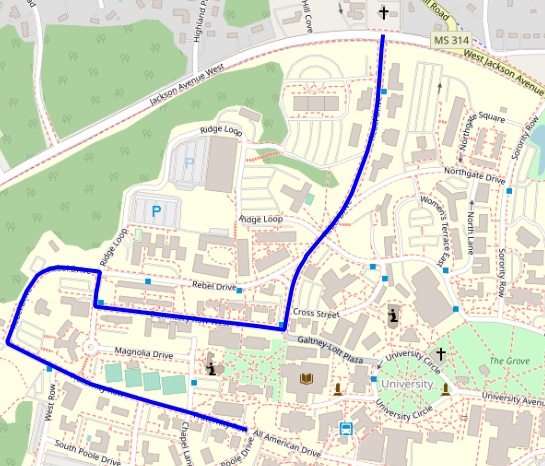
\includegraphics[width=\linewidth]{bfsc.png}
        \caption{Breath First Search.}
        \label{fig:bfs}
    \end{subfigure}
    \begin{subfigure}[b]{0.4\linewidth}
        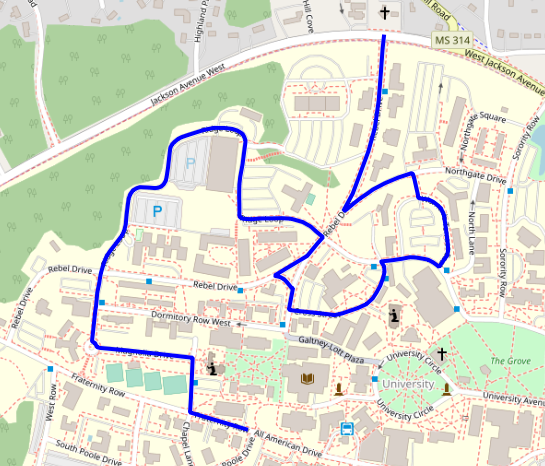
\includegraphics[width=\linewidth]{dfsc.png}
        \caption{Depth First Search.}
        \label{fig:dfs}
    \end{subfigure}
    \caption{Difference between DSF and BFS.}
    \label{fig:difference}
\end{figure}


\printbibliography

\end{document}